\documentclass[11pt,accentcolor=tud2a,colorback,noheadingspace,bigchapter]{tudreport}

\usepackage[utf8]{inputenc}
\usepackage{hyperref}
\usepackage{booktabs}
\usepackage{ltablex}
\usepackage{tabularx}
\usepackage{float}


\usepackage{enumitem}
\setlist[itemize]{parsep=0pt}
\setlist[description]{parsep=0.5\baselineskip}
\setlength\parindent{0pt}

\date{July 28, 2015}
\author{Thomas Gossmann}

\title{FVF Documentation}
\subtitle{Thomas Gossmann}
\subsubtitle{\hfill 28. Juli 2015}
\institution{Institut für Sportwissenschaft}
\setinstitutionlogo{ifslogo.png}

\newcommand{\code}[1]{\texttt{#1}}

\begin{document}

\maketitle
%\frontmatter

\begin{abstract}
The Flicker Fusion Frequency (FVF) is used to measure central nervous activation. 
This is the technical documentation for the measurement system. Reach for the 
\href{https://fvf-manual.readthedocs.org}{manual} on how to run your own tests.

The \href{http://www.sport.tu-darmstadt.de/sportinstitut/personal/professoren/wiemeyer\_seiten/forschung\_detail/forschung\_flimmerverschmelzungsfrequenz.de.jsp}{FVF measurement system} 
is created at the Institute for Sport Science at Technical University Darmstadt.
\end{abstract}

\setcounter{tocdepth}{1}
\tableofcontents

%\mainmatter
\part{About}

\chapter{Authors}
\label{about/authors:welcome-to-the-fvf-measurement-system-documentation}\label{about/authors::doc}\label{about/authors:authors}
The FVF measurement system is built by:

Project lead:
\begin{itemize}
\item
\href{http://www.sport.tu-darmstadt.de/sportinstitut/personal/professoren/wiemeyer\_seiten/wiemeyer\_profil.de.jsp}{Prof. Dr. Josef Wiemeyer}

\end{itemize}

Project members:
\begin{itemize}
\item Leonie Poetsch
\item Gerrit Kollegger
\item Thomas Gossmann
\end{itemize}

\chapter{License}
\label{about/license::doc}\label{about/license:license}
The MIT License (MIT)

Copyright (c) 2015 Thomas Gossmann

Permission is hereby granted, free of charge, to any person obtaining a copy
of this software and associated documentation files (the ``Software''), to deal
in the Software without restriction, including without limitation the rights
to use, copy, modify, merge, publish, distribute, sublicense, and/or sell
copies of the Software, and to permit persons to whom the Software is
furnished to do so, subject to the following conditions:

The above copyright notice and this permission notice shall be included in all
copies or substantial portions of the Software.

THE SOFTWARE IS PROVIDED ``AS IS'', WITHOUT WARRANTY OF ANY KIND, EXPRESS OR
IMPLIED, INCLUDING BUT NOT LIMITED TO THE WARRANTIES OF MERCHANTABILITY,
FITNESS FOR A PARTICULAR PURPOSE AND NONINFRINGEMENT. IN NO EVENT SHALL THE
AUTHORS OR COPYRIGHT HOLDERS BE LIABLE FOR ANY CLAIM, DAMAGES OR OTHER
LIABILITY, WHETHER IN AN ACTION OF CONTRACT, TORT OR OTHERWISE, ARISING FROM,
OUT OF OR IN CONNECTION WITH THE SOFTWARE OR THE USE OR OTHER DEALINGS IN THE
SOFTWARE.


\chapter{Contribute}
\label{about/contribute:contribute}\label{about/contribute::doc}
There are a couple of ways to contribute:
\begin{enumerate}
\item Create an \href{https://github.com/tudifs/fvf/issues}{issue} on github, if you realized something is wrong
\item You may clone the repo and send a pull-request which contains the fix
\item Get in {\hyperref[about/authors::doc]{\emph{\emph{contact}}}} with the team
\end{enumerate}
\part{Source}

\chapter{Structure}
\label{source/structure::doc}\label{source/structure:issue}\label{source/structure:structure}
The FVF measurement system is split into various pieces and components.


\section{Pieces}
\label{source/structure:pieces}
The FVF measurement system consists of multiple pieces:
\begin{itemize}
\item {}
Tube

\item {}
Hardware LED controller (Arduino Uno)

\item {}
Client Software

\end{itemize}


\section{Components}
\label{source/structure:components}
The software consists of multiple components written in multiple programming languages:
\begin{itemize}
\item {}
Arduino {\hyperref[source/firmware::doc]{\emph{\emph{Firmware}}}} (C++)

\item {}
LED {\hyperref[source/driver::doc]{\emph{\emph{Driver}}}} (Java)

\item {}
Client {\hyperref[source/software::doc]{\emph{\emph{Software}}}} (Java)

\end{itemize}


\section{Folders}
\label{source/structure:folders}
The folders and what they contain in this repository:
\begin{itemize}
\item {}
\code{docs/} - contains the source files for this documentation

\item {}
\code{driver/} - contains the source files for the {\hyperref[source/driver::doc]{\emph{\emph{Driver}}}}

\item {}
\code{firmware/} - contains the sources files for the {\hyperref[source/firmware::doc]{\emph{\emph{Firmware}}}}

\item {}
\code{software/} - contains the sources files for the {\hyperref[source/software::doc]{\emph{\emph{Software}}}}

\item {}
\code{manual/} - contains the sources files for the manual

\end{itemize}


\chapter{Firmware}
\label{source/firmware:firmware}\label{source/firmware::doc}
The firmware runs on the \textbf{Arduino Uno} board. The board is connected via an Universal Serial Port (USB) to the host computer which runs the measurement software. It's main job is to handle incoming commands (via serial port) and send back feedback notifications.


\section{Available Commands}
\label{source/firmware:available-commands}\begin{itemize}
\item {}
{\hyperref[appendix/led-protocol:protocol-input-on]{\emph{on}}}

\item {}
{\hyperref[appendix/led-protocol:protocol-input-flicker]{\emph{flicker}}}

\item {}
{\hyperref[appendix/led-protocol:protocol-input-off]{\emph{off}}}

\item {}
{\hyperref[appendix/led-protocol:protocol-input-measurement]{\emph{measurement}}}

\item {}
{\hyperref[appendix/led-protocol:protocol-input-ping]{\emph{ping}}}

\end{itemize}

Detailed information about the input and output about the firmware is described in the {\hyperref[appendix/led-protocol::doc]{\emph{\emph{LED Protocol}}}}.


\section{References}
\label{source/firmware:references}\begin{itemize}
\item {}
\href{http://www.arduino.cc/}{Arduino Website}

\item {}
\href{http://www.arduino.cc/en/Main/Software}{Arudino IDE}

\item {}
\href{http://www.arduino.cc/en/Reference/HomePage}{Arduino API}

\end{itemize}


\section{Verification}
\label{source/firmware:arduino-api}\label{source/firmware:verification}
To ensure the flickering frequency a verification measurement has been done with VOLTCRAFT Universal SYSTEM MS-9150 Frequency Counter.

An important Note: The \href{http://www.arduino.cc/en/Reference/Delay}{delay()} method on the Arduino passes the delay in integer values, no floats are possible. For every milliseconds below 16383, \href{http://www.arduino.cc/en/Reference/DelayMicroseconds}{delayMicroseconds()} must be used. The gap happens between 30Hz and 31Hz.


\subsection{Methodology}
\label{source/firmware:methodology}\label{source/firmware:delaymicroseconds}
Voltage has been captured at the pins directly at the measured LED. Each frequency was measured two times and the latter value was used.

Note: Prior sample measurements showed, the value didn't changed after the second measurement for each frequency.

\subsection{Results}
\label{source/firmware:results}

Results are shown in table~\ref{table:firmware-verification}.

\begin{tabularx}{\textwidth}{lll}
\caption{Measurement Results for Flicker-Frequency Accuracy Verification}
\label{table:firmware-verification}
\medskip
\hline
{\bf Frequency} & {\bf Measured Frequency} & {\bf Offset} \\
\hline
\endhead

10Hz
 &
9,996
 &
-0,004
\\

11Hz
 &
11,105
 &
+0,105
\\

12Hz
 &
12,186
 &
+0,185
\\

13Hz
 &
13,146
 &
+0,146
\\

14Hz
 &
14,270
 &
+0,270
\\

15Hz
 &
15,071
 &
+0,071
\\

16Hz
 &
16,110
 &
+0,110
\\

17Hz
 &
17,220
 &
+0,220
\\

18Hz
 &
18,488
 &
+0,488
\\

19Hz
 &
19,200
 &
+0,200
\\

20Hz
 &
19,966
 &
-0,034
\\

21Hz
 &
21,567
 &
+0,567
\\

22Hz
 &
22,678
 &
+0,678
\\

23Hz
 &
23,756
 &
+0,756
\\

24Hz
 &
24,935
 &
+0,935
\\

25Hz
 &
24,941
 &
-0,059
\\

26Hz
 &
26,245
 &
+0,245
\\

27Hz
 &
27,704
 &
+0,704
\\

28Hz
 &
29,191
 &
+1,191
\\

29Hz
 &
29,196
 &
+0,196
\\

30Hz
 &
31,138
 &
+1,138
\\

31Hz
 &
30,772
 &
-0,328
\\

32Hz
 &
31,723
 &
-0,277
\\

33Hz
 &
32,712
 &
-0,288
\\

34Hz
 &
33,702
 &
-0,298
\\

35Hz
 &
34,689
 &
-0,311
\\

36Hz
 &
35,673
 &
-0,327
\\

37Hz
 &
36,657
 &
-0,343
\\

38Hz
 &
37,646
 &
-0,354
\\

39Hz
 &
38,633
 &
-0,367
\\

40Hz
 &
39,621
 &
-0,379
\\

41Hz
 &
40,598
 &
-0,402
\\

42Hz
 &
41,590
 &
-0,41
\\

43Hz
 &
42,578
 &
-0,422
\\

44Hz
 &
43,562
 &
-0,438
\\

45Hz
 &
44,544
 &
-0,456
\\

46Hz
 &
45,275
 &
-0,725
\\

47Hz
 &
46,520
 &
-0,48
\\

48Hz
 &
47,500
 &
-0,5
\\

49Hz
 &
48,481
 &
-0,519
\\

50Hz
 &
49,465
 &
-0,536
\\

51Hz
 &
50,454
 &
-0,546
\\

52Hz
 &
51,436
 &
-0,564
\\

53Hz
 &
52,414
 &
-0,586
\\

54Hz
 &
53,152
 &
-0,848
\\

55Hz
 &
54,389
 &
-0,611
\\

...
 &  & \\

500Hz
 &
468,991
 &
-32,009
\\
\hline
\end{tabularx}


Figure~\ref{fig:firmware-verification} graph shows the scattering of the measured values around the expected linear ideal values.

\begin{figure}[H]
	\centering
	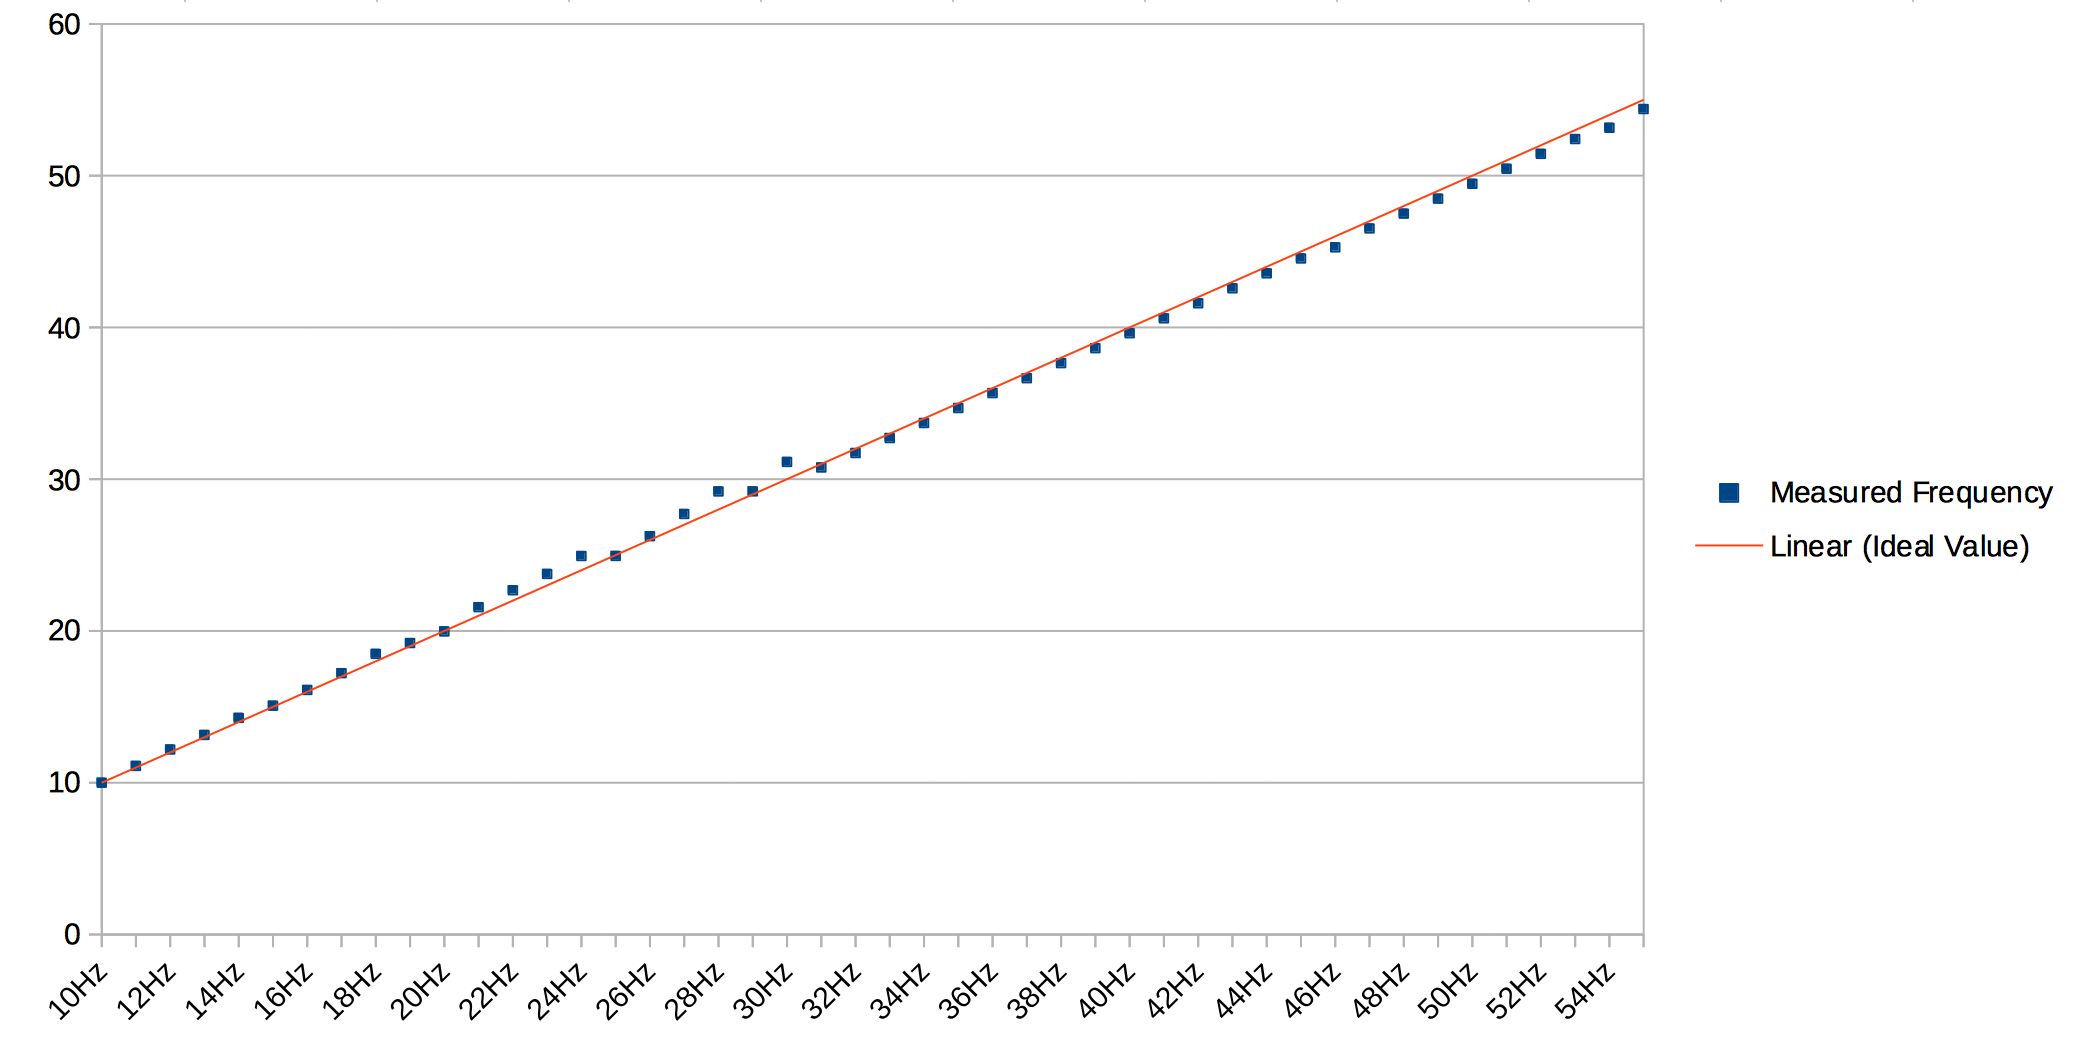
\includegraphics[width=\textwidth]{images/firmware-verification.png}
	\caption{Measurement Results for Flicker-Frequency Accuracy Verification with Frequency Line}
	\label{fig:firmware-verification}
\end{figure}


\chapter{Driver}
\label{source/driver:driver}\label{source/driver::doc}
The LED driver is a Java API to send commands to the {\hyperref[source/firmware::doc]{\emph{\emph{Firmware}}}} and getting notified about feedback from the firmware.


\section{Communication}
\label{source/driver:communication}
The client software talks to the Arduino board through a serial port connection. For this purpose the RXTX interface is used. In order to check whether the connection is still established, the driver periodically sends a ping to the board. Once this connection is interrupted for several reasons, it's assumed the connection is dead.


\section{Protocol}
\label{source/driver:protocol}
The driver implements the {\hyperref[appendix/led-protocol::doc]{\emph{\emph{LED Protocol}}}}.


\section{Deployment}
\label{source/driver:deployment}
The driver is deployed as \code{*.jar} file into the softwares \code{lib/} folder.

\begin{figure}[H]
	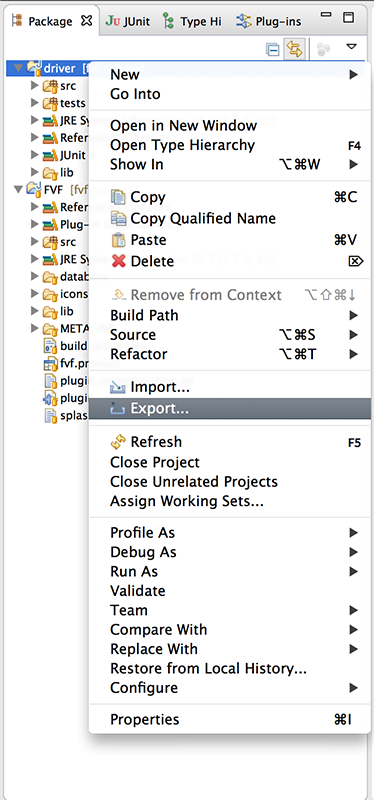
\includegraphics[width=0.45\textwidth]{images/driver_export.png}
	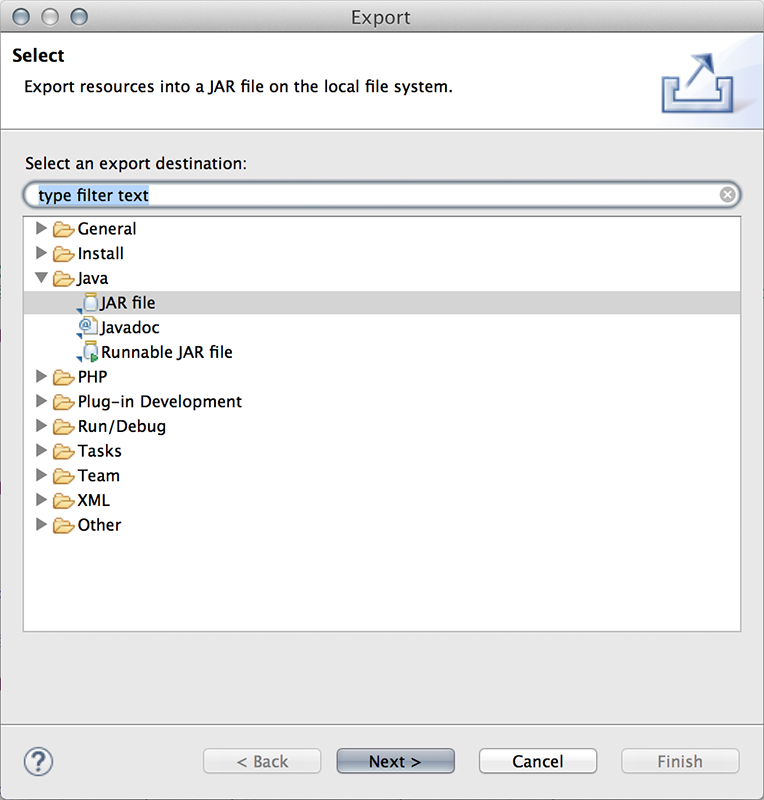
\includegraphics[width=0.45\textwidth]{images/driver_export_dialog.png}
	\caption{Deploy as jar}
	\label{fig:deployment-driver}
\end{figure}

Note: This is not ideal and must be triggered manually. Better solutions are welcome.


\section{Remarks}
\label{source/driver:remarks}
There is a \href{http://rxtx.qbang.org/wiki/index.php/Wrapping\_RXTX\_in\_an\_Eclipse\_Plugin}{rxtx wiki entry} describing how to bundle the jni extension with an eclipse rcp application.


\subsection{Mac OS X}
\label{source/driver:rxtx-wiki-entry}\label{source/driver:mac-os-x}
The normal distributed \code{librxtxSerial.jnilib} is only in 32-bit mode which doesn't match a 64-bit processor architecture and can thus not be autoloaded. See here:

\begin{verbatim}
$ file librxtxSerial.jnilib
librxtxSerial.jnilib: Mach-O universal binary with 2 architectures
librxtxSerial.jnilib (for architecture ppc):  Mach-O dynamically linked shared library ppc
librxtxSerial.jnilib (for architecture i386): Mach-O dynamically linked shared library i386
\end{verbatim}

Luckily there is a 64-bit version available, forged by \href{http://blog.iharder.net/2009/08/18/rxtx-java-6-and-librxtxserial-jnilib-on-intel-mac-os-x/}{Robert Harder}. The eclipse plugin distributes the 64-bit version mentioned here:

\begin{verbatim}
$ file librxtxSerial.jnilib
librxtxSerial.jnilib: Mach-O universal binary with 4 architectures
librxtxSerial.jnilib (for architecture x86_64):       Mach-O 64-bit bundle x86_64
librxtxSerial.jnilib (for architecture i386): Mach-O bundle i386
librxtxSerial.jnilib (for architecture ppc7400):      Mach-O bundle ppc
librxtxSerial.jnilib (for architecture ppc64):        Mach-O 64-bit bundle ppc64
\end{verbatim}


\subsection{Disconnecting}
\label{source/driver:robert-harder}\label{source/driver:disconnecting}
There are some problems between RXTX and properly disconnecting connections. The problems are described in a \href{http://archive.infiniteautomation.com/forum/posts/list/297.page}{forum thread}. The mentioned hacks are implemented precautionally. Probably RXTX version 2.2 should have these issues resolved, yet wasn't available stable at the time of implementation.


\section{References}
\label{source/driver:forum-thread}\label{source/driver:references}\begin{itemize}
\item {}
\href{http://rxtx.qbang.org}{RXTX}

\item {}
\href{http://playground.arduino.cc/Interfacing/Java}{Arduino Java Interface}

\end{itemize}


\chapter{Software}
\label{source/software:arduino-java-interface}\label{source/software::doc}\label{source/software:software}
The heart of the measurement system is the software, which is responsible for managing your probands, running tests and browsing the results. It is an \href{http://eclipse.org/rcp}{Eclipse RCP} application. It uses the eclipse e3 API. Latest API docs are available at \href{http://help.eclipse.org}{Eclipse Help}.


\section{Database}
\label{source/software:eclipse-help}\label{source/software:database}
Database development is realized via \href{http://sormula.org}{sormula} ORM. 
The models are located in the \\ \code{de.tu\_darmstadt.sport.fvf.model} package. 
The respective {\hyperref[appendix/erm::doc]{\emph{\emph{ERM}}}} is available as appendix. It is a SQLite database which is realized with \href{http://sqljet.com}{SQLJet} and connected with \href{http://www.xerial.org/trac/Xerial/wiki/SQLiteJDBC}{SQLite JDBC}.


\subsection{Migrations}
\label{source/software:sqlite-jdbc}\label{source/software:migrations}
Further version might require a migration of the underlying database. The mechanics for this are already implemented and ready to use. SQLJet allows to stores a user version number along with the database file. The purpose is to read this number at start and run a migration if necessary. The class \code{de.tu\_darmstadt.sport.fvf.database.DatabaseLoader} handles this logic. The required code to read the version number is already available in the \code{initialize()} method, yet commented out but provides good start.


\section{Icons}
\label{source/software:icons}
Icons are \href{http://www.famfamfam.com/lab/icons/silk/}{Silk} by famfamfam and \href{http://p.yusukekamiyamane.com}{Fugue} by Yusuke Kamiyamane.
\phantomsection\label{index:dev-docs}

\part{Developer}

\chapter{Setup}
\label{development/setup:fugue}\label{development/setup:setup}\label{development/setup::doc}
Learn how to setup your development environment for FVF.


\section{Installing Arduino}
\label{development/setup:installing-arduino}
Installing the Arduino IDE is straight forward. From the \href{http://www.arduino.cc/en/Main/Software}{Arduino Website} download the Arduino IDE for your platform and open \code{firmware/fvf/fvf.ino} to start your firmware development.


\subsection{Arduino Drivers}
\label{development/setup:arduino-drivers}\label{development/setup:arduino-website}
Some systems require a manual driver installation for the Arduino board. Please refer to the \href{http://www.arduino.cc/en/Guide/HomePage}{Getting Started Guide} from the Arduino website if this is required for you and how to get this done.


\subsection{CoolTerm}
\label{development/setup:coolterm}\label{development/setup:getting-started-guide}
\href{http://freeware.the-meiers.org/}{CoolTerm} is a simple serial port terminal application. CoolTerm can be used to send commands to the Arduino Board and test your firmware.


\section{Install Git}
\label{development/setup:install-git}\label{development/setup:id1}
Git is used as VCS and GitHub as repository master.


\subsection{Windows}
\label{development/setup:windows}
Luckily GitHub provides an application with GUI to access git repositories. \href{https://windows.github.com/}{Download GitHub for Windows} and install it; Clone the repo from GitHub and you are ready to go.


\subsection{Mac}
\label{development/setup:download-github-for-windows}\label{development/setup:mac}
Also Mac got a GitHub app with GUI to access git repositories. \href{https://mac.github.com/}{Download GitHub for Mac} and install it; Clone the repo from GitHub and you are ready to go.


\subsection{Linux}
\label{development/setup:download-github-for-mac}\label{development/setup:linux}
You are on Linux, you know how to use your personal package manager to install yourself a git package and of course you can handle it from your favorite shell.


\section{Installing Eclipse}
\label{development/setup:installing-eclipse}
Eclipse is the main development environment. A good start is to download the \href{https://www.eclipse.org/downloads/}{Eclipse for RCP and RAP Developers} package.


\subsection{Install PDE Tools}
\label{development/setup:install-pde-tools}\label{development/setup:eclipse-for-rcp-and-rap-developers}
To help and assist you with programming (Javadoc + proper code completion), install the following plugins from ``The Eclipse Project and Updates'' update site (Help \textgreater{} Install New Software ... Update Site: \href{http://download.eclipse.org/eclipse/updates/4.4}{http://download.eclipse.org/eclipse/updates/4.4} - replace ``4.4'' with the current version number):
\begin{itemize}
\item {} 
Eclipse Plug-In Development Environment

\item {} 
Eclipse Platform SDK

\item {} 
Eclipse Java Development Tools

\end{itemize}

Note: Some of them might already be installed.


\subsection{Install Deployment Tools}
\label{development/setup:setup-deltapack}\label{development/setup:install-deployment-tools}
To deploy the FVF application bundle to multiple platforms the eclipse ``DeltaPack'' is required for this.
Read here for installation: \href{https://stackoverflow.com/a/12737382/483492}{https://stackoverflow.com/a/12737382/483492}


\subsection{Install Optional Tools}
\label{development/setup:install-optional-tools}
There are more useful plug-ins to support your development. They are available via the current releases update site (Help \textgreater{} Install New Software ... Update Site: \href{http://download.eclipse.org/releases/luna}{http://download.eclipse.org/releases/luna} - replace ``luna'' with the current release):
\begin{itemize}
\item {} 
SWT Designer

\item {} 
Eclipse GIT Team provider

\end{itemize}


\chapter{Deployment}
\label{development/deployment::doc}\label{development/deployment:deployment}
This page describes, how to deploy your own version of the measurement software.


\section{Required Plugins}
\label{development/deployment:required-plugins}
Since this is an e3 Plug-In deployed in an e4 environment all required \href{https://www.eclipse.org/community/eclipse\_newsletter/2013/february/article3.php\#compatibiliylayer\_plugins}{compatibility layer plugins} must be added.


\section{Export the RCP application}
\label{development/deployment:export-the-rcp-application}\label{development/deployment:compatibility-layer-plugins}
Open the \code{fvf.product} file in eclipse. On the \emph{Overview} page there is the export section with a link to open the ``Eclipse Product export wizard'' (which is also available from the toolbar of this editor). Make sure to check ``Export for multiple platforms'' (which is only available if you followed the {\hyperref[development/setup:setup-deltapack]{\emph{Install Deployment Tools}}} instructions) and ``Synchronize before exporting''. Click ``Next'' which shows the available platforms to deploy to.


\chapter{Documentation}
\label{development/documentation:documentation}\label{development/documentation::doc}
The process of writing documentation is also known as \emph{continuous documentation}. The raw source files are written in \href{http://docutils.sourceforge.net/rst.html}{reStructuredText} and \href{http://sphinx-doc.org}{Sphinx} is used to generate the documentation in various formats. \href{http://readthedocs.org}{Read the Docs} hosts this documentation.


\chapter{Follow-Up Projects}
\label{development/follow-ups::doc}\label{development/follow-ups:sphinx}\label{development/follow-ups:follow-up-projects}
Some ideas for follow-up projects.


\section{Automated Builds}
\label{development/follow-ups:automated-builds}
Currently deploying the software is a manual job. It would be more pleasant to have automated builds. This especially means two tasks:
\begin{enumerate}
\item {} 
Driver and FVF are two independent projects right now, which means deploying the driver first to use it from FVF, it would be way easier to just refer to the driver project instead.

\item {} 
Deploy the software (with all it's required libs). Either automatically, by committing, tagging a release or trigger the build manually.

\end{enumerate}

For option \#2 (continuous deployment) there are some online services available, which must be checked individually if they are eligible for the task on hand:
\begin{itemize}
\item {} 
\href{https://semaphoreci.com}{semaphore}

\item {} 
\href{https://codeship.com}{codeship}

\item {} 
\href{http://dploy.io}{dploy}

\item {} 
\href{https://drone.io}{drone.io}

\item {} 
\href{https://circleci.com}{circleci}

\end{itemize}

Additionally, there must be found a good place to distribute binaries to.


\section{Streamline Web Presence}
\label{development/follow-ups:streamline-web-presence}
The current web presence is cluttered among this \href{https://fvf.readthedocs.org}{docs} and the \href{https://fvf-manual.readthedocs.org}{manual}. A formal webpage introducing FVF, what it is, who is responsible for that, where to download, how to contribute and contains links to the docs and manual is missing. Probably \href{https://pages.github.com}{GitHub pages} are a solution to island this or possibly put this up on the \href{http://www.sport.tu-darmstadt.de}{IFS website}.


\section{Internationalization (i18n)}
\label{development/follow-ups:internationalization-i18n}\label{development/follow-ups:ifs-website}
Right now, the docs are in english, software and manual are in german. All tools within the toolchain support internationalization. This can be used to better translate all occurring strings. \href{https://www.transifex.com}{Transifex} is an online service to keep track of all translations, which can be used as a managing instance. There is even an integration between Transifex and Sphinx, to \href{http://sphinx-doc.org/intl.html}{translate docs}.


\section{Self-Validation}
\label{development/follow-ups:self-validation}\label{development/follow-ups:translate-docs}
A self-validation routine built into the {\hyperref[source/firmware::doc]{\emph{\emph{Firmware}}}} that averages the deviation for each frequency and applies it during the measurement routine.


\section{Post-Processing of Results}
\label{development/follow-ups:post-processing-of-results}
The results can receive some post-processing by either showing statistics and displaying graphs or providing exports to various formats for further processing, e.g. exporting to SPS.


\section{Instructions to setup your own FVF measurement system}
\label{development/follow-ups:instructions-to-setup-your-own-fvf-measurement-system}
Instructions to setup one's own FVF measurement system. With technical specifications of the tube and the oculus adapter to connecting the software. Likewise a step-by-step manual for a self-construction-kit.


\section{Port to eclipse e4}
\label{development/follow-ups:port-to-eclipse-e4}
For historical reasons, the software is built on eclipse e3 API. At the time of writing, e4 is the current API and contains modern programming approaches to simply development. It can be worth to port the codebase to the new e4 API.
\phantomsection\label{index:appendix-docs}

%\backmatter
\part{Appendix}

\chapter{LED Protocol}
\label{appendix/led-protocol:led-protocol}\label{appendix/led-protocol::doc}
The firmware communicates with the protocol described here. The driver sends a command with arguments ({\hyperref[appendix/led-protocol:protocol-input]{\emph{Input}}}) and the hardware send feedback on what is happening ({\hyperref[appendix/led-protocol:protocol-output]{\emph{Output}}}).


\section{Schema}
\label{appendix/led-protocol:schema}
The following schema is used for every command, in every direction:

\begin{verbatim}
cmd [arg1] [arg2] ... [argN]
\end{verbatim}


\section{Input}
\label{appendix/led-protocol:input}\label{appendix/led-protocol:protocol-input}
Commands send to the hardware


\subsection{on}
\label{appendix/led-protocol:on}\label{appendix/led-protocol:protocol-input-on}
Turns on a led:

\begin{verbatim}
on [led]
\end{verbatim}

\textbf{Arguments}
\begin{itemize}
\item {} 
\code{led} (int) - the led number

\end{itemize}


\subsection{flicker}
\label{appendix/led-protocol:flicker}\label{appendix/led-protocol:protocol-input-flicker}
Flickers a led:

\begin{verbatim}
flicker [led] [frequency] [duration] [[light]] [[dark]]
\end{verbatim}

\textbf{Arguments}
\begin{itemize}
\item {} 
\code{led} (int) - the led number

\item {} 
\code{frequency} (int) - the flicker frequency {[}hz{]}

\item {} 
\code{duration} (int) - the duration the led flickers {[}ms{]}

\item {} 
\code{light} (int) - the light part of the light/dark ratio (optional)

\item {} 
\code{dark} (int) - the dark part of the light/dark ratio (optional)

\end{itemize}


\subsection{off}
\label{appendix/led-protocol:protocol-input-off}\label{appendix/led-protocol:off}
Turns off a led:

\begin{verbatim}
off [led]
\end{verbatim}

\textbf{Arguments}
\begin{itemize}
\item {} 
\code{led} (int) - the led number

\end{itemize}


\subsection{measurement}
\label{appendix/led-protocol:protocol-input-measurement}\label{appendix/led-protocol:measurement}
Runs a measurement sequence:

\begin{verbatim}
measurement [mode] [flickerLed] [frequency] [onDuration] [offDuration]
\end{verbatim}

\textbf{Arguments}
\begin{itemize}
\item {} 
\code{mode} (int) - \emph{2} for two leds and \emph{4} for four leds

\item {} 
\code{flickerLed} (int) - Which led will flicker

\item {} 
\code{frequency} (float) - The frequency for the flickering led {[}hz{]}

\item {} 
\code{onDuration} (int) - The duration, the leds will be on {[}ms{]}

\item {} 
\code{offDuration} (int) - The duration, the leds will be off {[}ms{]}

\end{itemize}


\subsection{ping}
\label{appendix/led-protocol:ping}\label{appendix/led-protocol:protocol-input-ping}
Sends a ping:

\begin{verbatim}
ping [[seq]]
\end{verbatim}

\textbf{Arguments}
\begin{itemize}
\item {} 
\code{seq} (misc) - An optional sequence identifier (optional)

\end{itemize}


\section{Output}
\label{appendix/led-protocol:output}\label{appendix/led-protocol:protocol-output}
Feedback received from the hardware.


\subsection{on}
\label{appendix/led-protocol:protocol-output-on}\label{appendix/led-protocol:id1}
Send when a led is turned on (or flickering, when measurement command was used):

\begin{verbatim}
on [led]
\end{verbatim}

\textbf{Arguments}
\begin{itemize}
\item {} 
\code{led} (int) - the led number

\end{itemize}


\subsection{flicker}
\label{appendix/led-protocol:id2}\label{appendix/led-protocol:protocol-output-flicker}
Send when a led is flickering:

\begin{verbatim}
flicker [led]
\end{verbatim}

\textbf{Arguments}
\begin{itemize}
\item {} 
\code{led} (int) - the led number

\end{itemize}


\subsection{off}
\label{appendix/led-protocol:protocol-output-off}\label{appendix/led-protocol:id3}
Send when a led is turned off:

\begin{verbatim}
off [led]
\end{verbatim}

\textbf{Arguments}
\begin{itemize}
\item {} 
\code{led} (int) - the led number

\end{itemize}


\subsection{measurement}
\label{appendix/led-protocol:id4}\label{appendix/led-protocol:protocol-output-measurement}
Send when a measurement is started or finished:

\begin{verbatim}
measurement [state]
\end{verbatim}

\textbf{Arguments}
\begin{itemize}
\item {} 
\code{state} (string) - \code{on} when the measurement started and \code{off} when it's finished

\end{itemize}


\subsection{ons}
\label{appendix/led-protocol:ons}\label{appendix/led-protocol:protocol-output-ons}
Send when more than one led is turned on (during a measurement):

\begin{verbatim}
ons [mode]
\end{verbatim}

\textbf{Arguments}
\begin{itemize}
\item {} 
\code{mode} (int) - is either 2 or 4, depending the first value of the \code{measurement} input command

\end{itemize}


\subsection{offs}
\label{appendix/led-protocol:protocol-output-offs}\label{appendix/led-protocol:offs}
Send when more than one led is turned off (during a measurement):

\begin{verbatim}
offs [mode]
\end{verbatim}

\textbf{Arguments}
\begin{itemize}
\item {} 
\code{mode} (int) - is either 2 or 4, depending the first value of the \code{measurement} input command

\end{itemize}


\subsection{pong}
\label{appendix/led-protocol:pong}\label{appendix/led-protocol:protocol-output-pong}
Answers a ping with a pong:

\begin{verbatim}
pong [seq]
\end{verbatim}

\textbf{Arguments}
\begin{itemize}
\item {} 
\code{seq} (misc) - The returned sequence identifier (optional)

\end{itemize}


\subsection{error}
\label{appendix/led-protocol:protocol-output-error}\label{appendix/led-protocol:error}
Send when an error occured:

\begin{verbatim}
error [number]
\end{verbatim}

\textbf{Arguments}
\begin{itemize}
\item {} 
\code{number} (int) - the error number (see below)

\end{itemize}


\section{Error Codes}
\label{appendix/led-protocol:error-codes}
Error code explanation:
\begin{itemize}
\item {} 
\emph{0} - Unknown Error

\item {} 
\emph{1} - Malformed command

\item {} 
\emph{2} - Unknown command

\item {} 
\emph{3} - Too few arguments for flicker command

\end{itemize}


\section{Troubleshooting}
\label{appendix/led-protocol:troubleshooting}
1. Getting a ``Port in Use'' exception on OSX, when connecting to the Arduino Board
-\textgreater{} See here: \href{https://marcosc.com/2011/10/arduino-java-error-serial-port-already-in-use/}{https://marcosc.com/2011/10/arduino-java-error-serial-port-already-in-use/}


\chapter{Entity-Relationship-Model}
\label{appendix/erm:erm}\label{appendix/erm::doc}
The softwares database entity-relationship-model (ERM) as seen in Figure~\ref{fig:appendix-erm}

\begin{figure}[H]
	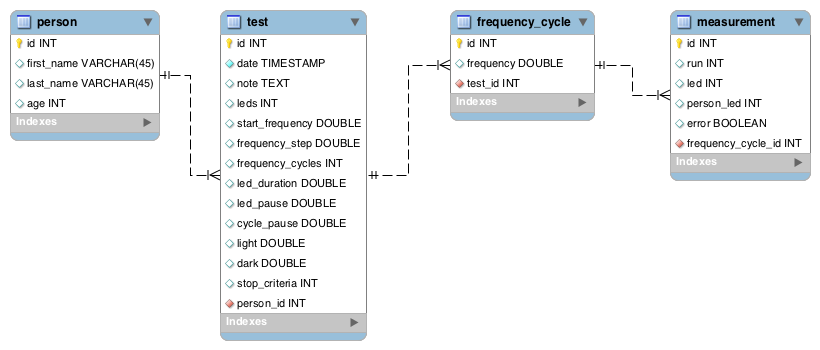
\includegraphics[width=\textwidth]{images/erm.png}
	\caption{ERM}
	\label{fig:appendix-erm}
\end{figure}



\end{document}
			